\documentclass[french,12pt]{article}
\usepackage{graphicx} % Required for inserting images
\usepackage{subfigure}
\usepackage{float}

% Set page size and margins
% Replace `letterpaper' with `a4paper' for UK/EU standard size
\usepackage[letterpaper,top=2cm,bottom=2cm,left=3cm,
right=3cm,marginparwidth=1.75cm]{geometry}
\usepackage{csquotes}

% Useful packages

\usepackage{fix-cm}% to provide smooth tiny font sizes
\usepackage{amsmath,mathtools}
\usepackage{bbm}
\usepackage{amsfonts}
\usepackage{graphicx}
% \usepackage{algpseudocode}
% \usepackage{algorithm}
\usepackage[ruled, lined]{algorithm2e}
\usepackage[colorlinks=true, allcolors=blue]{hyperref}

% Langue
% \usepackage[french]{babel}
\usepackage{babel}
\usepackage[T1]{fontenc}

% Redirection avec la table des matières
\hypersetup{
    colorlinks,
    citecolor=black,
    filecolor=black,
    linkcolor=black,
    urlcolor=black
}

% Pour les scripts
\usepackage{listings}
\usepackage{xcolor}

\definecolor{codegreen}{rgb}{0,0.6,0}
\definecolor{codegray}{rgb}{0.5,0.5,0.5}
\definecolor{codepurple}{rgb}{0.58,0,0.82}
\definecolor{backcolour}{rgb}{0.95,0.95,0.92}

\lstdefinestyle{mystyle}{
    backgroundcolor=\color{backcolour},
    commentstyle=\color{codegreen},
    keywordstyle=\color{magenta},
    numberstyle=\tiny\color{codegray},
    stringstyle=\color{codepurple},
    basicstyle=\ttfamily\footnotesize,
    breakatwhitespace=false,
    breaklines=true,
    captionpos=b,
    keepspaces=true,
    numbers=left,
    numbersep=5pt,
    showspaces=false,
    showstringspaces=false,
    showtabs=false,
    tabsize=2
}

\lstset{style=mystyle}

\title{PFE}
\author{Khaled MEDJKOUH \\ Davidson Lova RAZAFINDRAKOTO}

\begin{document}

\maketitle

\pagebreak

\tableofcontents

\pagebreak

\section{Introduction}
Incertitudes utile dans plusieurs domaines et la quantification duquel
est nécessaire pour des évaluations de risques, déctection d'anomalie et prise décision.

\subsection{Réseau de neurones}

Un réseaux de neurones est composé d'une couché d'entrée, des couches cachés
et une couche de sortie.

\begin{figure}[H]
    \centerline{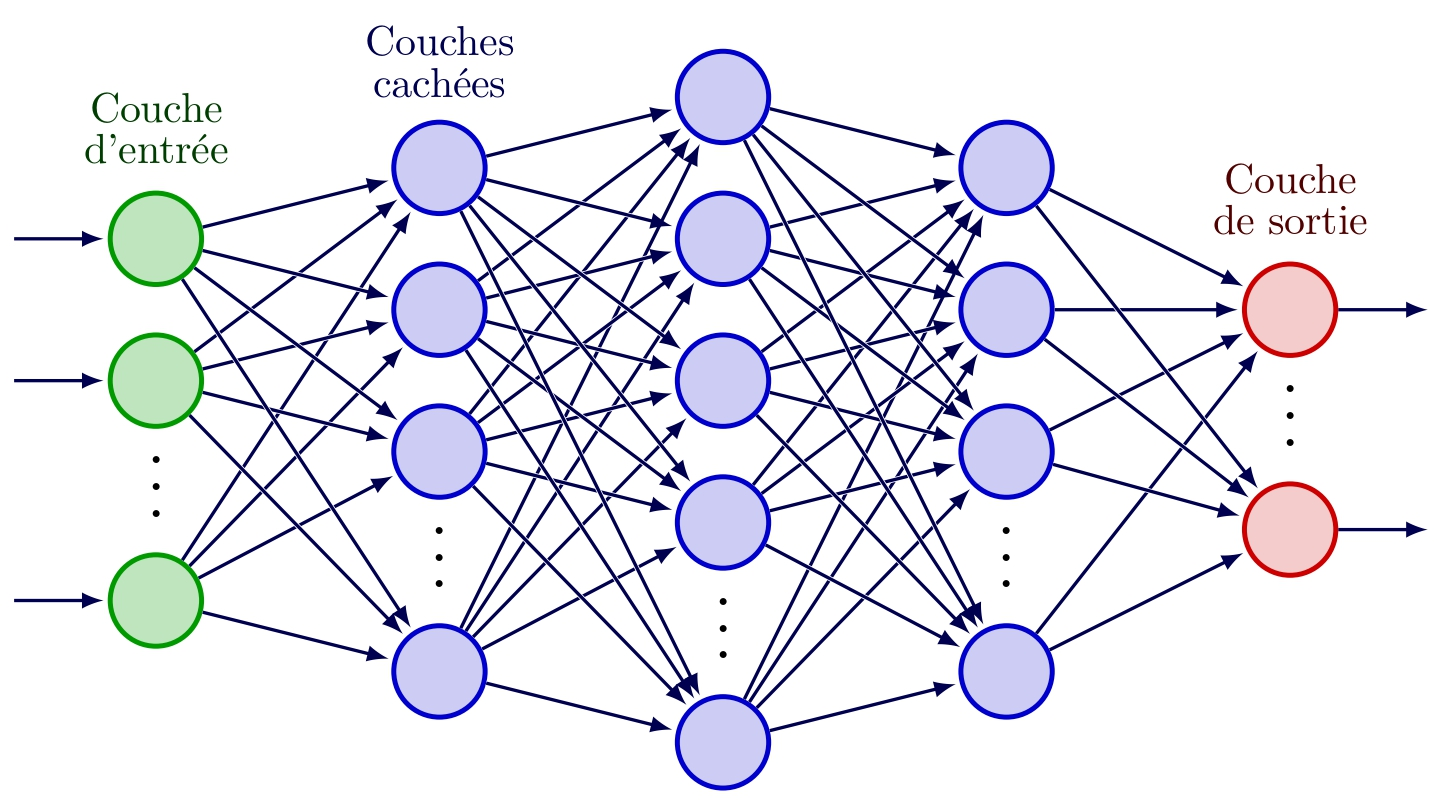
\includegraphics[width = 0.6\textwidth]{FNN/Images/fnn/fnn_page-0001.jpg}}
    \caption{Schéma de réseaux}
    \label{fig:fnn}
\end{figure}

La couche d'entrée prend la donnée d'entrée $x$, et la fait passer le long des couches cachées
pour finalement arrivée à la couche de sortie. Ci-dessous on voit comment sont évaluer les valeurs
pour chaque couche. 

\begin{figure}[H]
    \centerline{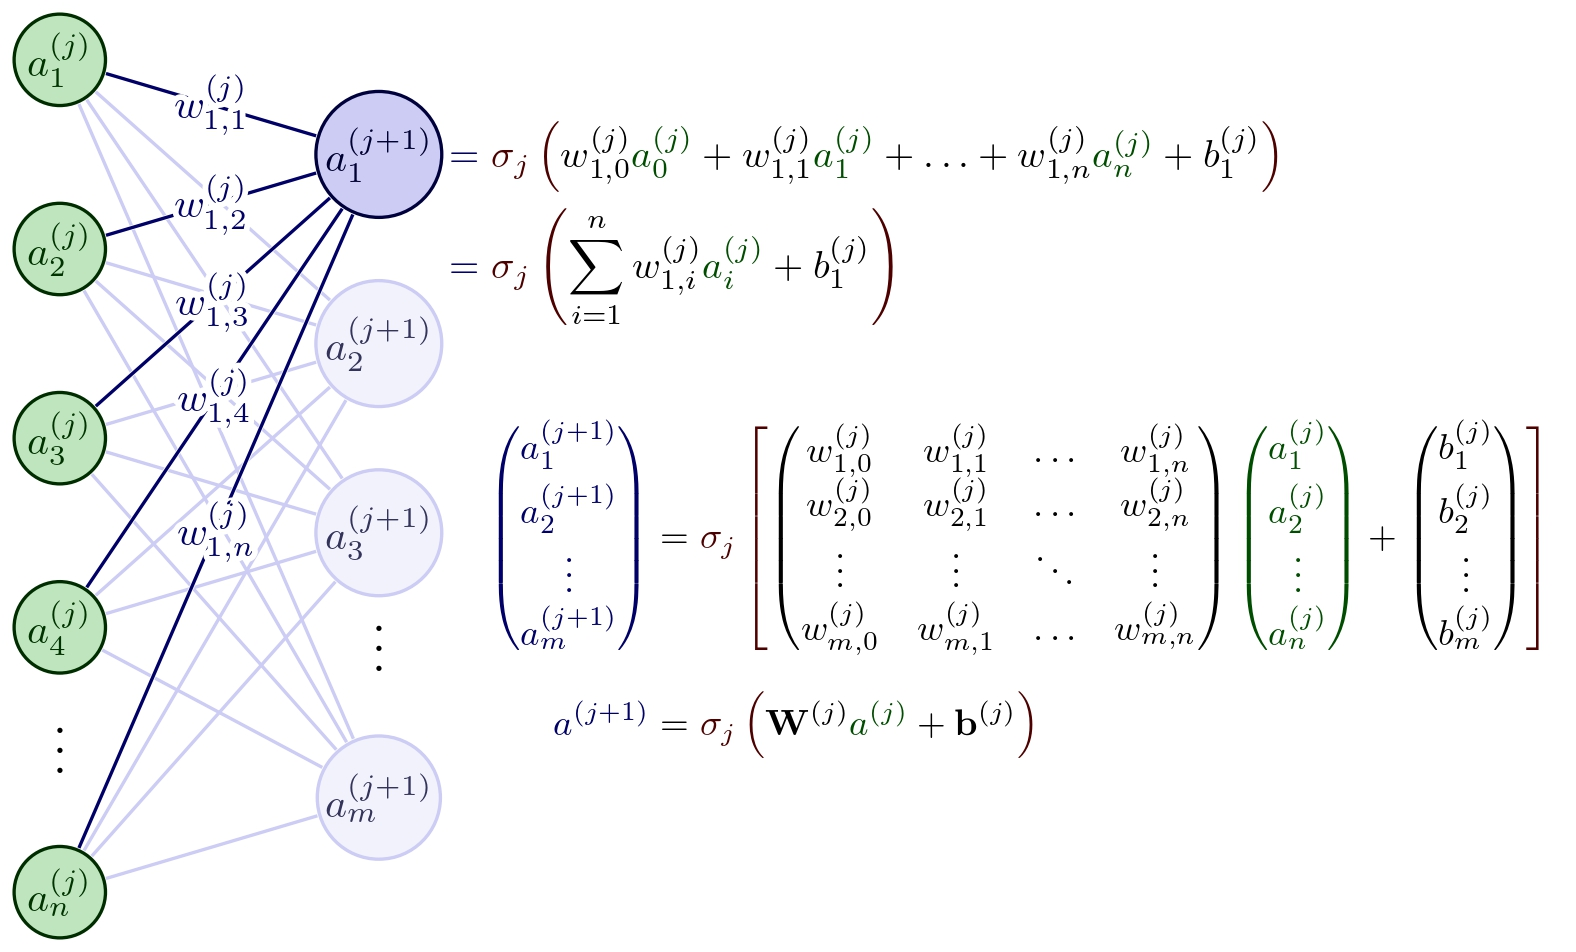
\includegraphics[width = 0.75\textwidth]{FNN/Images/fnnDetails/fnnDetails_page-0001.jpg}}
    \caption{Feed Forward}
    \label{fig:fnnDetails}
\end{figure}

+ Quelque résultats et application

+ Ce qui nous amène à un problème





\subsection{Source d'incertitudes dans un réseaux de neurones}

On modélise le réseaux de neurones comme la fonction non linéaire

$$f : (x, \theta) \in \mathcal{X} \times \Theta \mapsto f(x, \theta) \in \mathcal{Y}$$

où

\begin{itemize}
    \item $\mathcal{X} \subset \mathbb{R}^{n_e}$, l'espace des variables d'entrées
    \item $\mathcal{Y} \subset \mathbb{R}^{n_s}$, l'espace des variables de sorties
    \item $\Theta \subset \mathbb{R}^{n_p}$ , l'espace des paramètres
\end{itemize}

On se donne maintenant une base de données d'entrainement
$D = \{ (x_i, y_i)\}_{i = 1}^N \in (\mathcal{X} \times \mathcal{Y})^N$.

\subsubsection{Acquisition des données}
Si on prend comme données d'entrées $x$ une mesure d'une quantité réel $\tilde{x}$.

Il y a une variabilité sur la mesure en fonction des circonstances
et conditions $\omega \in \Omega$ dans lequel la mesure a été effectué.

La sortie $y$ peut aussi subir des erreurs de labelisation
(pour le cas d'une tâche de classification) ou aussi de mesure si c'est une quantité mesuré.

En somme on a une incertitude sur l'entrée $x | \omega \sim p_{x | \omega}$
et $y | \omega \sim p_{y | \omega}$.

S'ajoute à ça, l'incertitude sur $x$ qui peut se propager sur le $y$.

\subsubsection{Structure du model}

Les paramètres $\theta$ et donc l'espace $\Theta$ est variable en fonction du choix de model $s$.

On a $\theta | D,s \sim p_{\theta | D, s}$

\subsection{Prédiction}

La distribution de la prédiction $y^*$ sachant une entrée $x^*$ est données par

$$ p(y^* | x^*, D) = \int_{\Theta} \underbrace{p(y^* | x^*, \theta)}_{\text{Données}} \underbrace{p(\theta  | D)}_{\text{Modèle}} d \theta$$

\subsubsection{Incertitude aléatoire}

Insert definition here

Elle affecte la partie $p(y^* | x^*, \theta)$ de la tâche de prédiction,
elle est dus à la variabilité(précision et erreurs) lors des mesures.
Elle est donnée et inhérent au problème.

\subsubsection{Incertitude épistemique}

Insert definition here

Affecte la partie $p(\theta  | D)$ de la tâche de prédiction,
elle due :

\begin{itemize}
    \item à la compléxité du modèle,
    \item aux erreurs durant la phase d'entrainement,
    \item à la manque d'information à cause de données manquantes
          ou la capacité de représentation des donnés d'entrainement.
\end{itemize}

\pagebreak

\section{Réseau de neurones bayésiens (BNN)}

% + Présentation de réseaux de neurones bayésiens

Les réseaux de neurones bayésiens sont des réseaux de neurones
dont les poids sont, non pas des quantités déterministes (comme
dans le cas d'un NN normale) mais des distributions.

A l'initialisation, les poids suivent une loi a priori $p(\theta)$,
et l'entrainement consiste à évaluer l'a posteriori de cette loi conditionnée
aux données d'entrainement $p(\theta | D)$.

% + Donner son interet dans la résolution du problème précédent

% + Donner les méthodes d'entrainement d'un tel réseaux
On ne dispose pas dans le cas générale, d'une formule analytique de cette
distribution a posteriori.

Voici trois familles de méthodes pour approcher cette distribution :


\begin{itemize}
    \item Méthodes variationelle
    \item Méthodes par échantillonage ou
          Monte Carlo (qu'on va voir dans la suite)
    \item Méthodes de Laplace
\end{itemize}


\subsection{Méthodes variationelles}

Ici on approche $p(\theta | D)$ par une famille de distribution
paramétrique $\{q^{\gamma}(\theta)\}_{\gamma}$ (souvent des gaussiennes).
Le but est de choisir $\gamma$ qui rapproche $q^{\gamma}(\theta)$
le plus de $p(\theta | D)$. La distance choisit ici est la divergence
de Kullback-Leibler :

$$KL(q||p) = \mathbb{E}_q \left[\log \frac{q^{\gamma}(\theta)}{p(\theta | D)}\right]$$

Comme on ne connait pas $p(\theta | D)$, on utilise l'ELBO (evidence lower bound)
qui est égal à la divergence à une constante paramètres

$$L =\mathbb{E}_q \left[\log \frac{p(y | D, \theta)}{q^{\gamma}(\theta)}\right]$$

(on a en effet $KL(q||p) = -L +  \log p(y| D)$)

\subsection{Méthode de Laplace}

$\hat{\theta}$ l'estimateur de maximum d'a priori

$$\log p(\theta | D) \approx \log p(\hat{\theta} | D)
    + \frac{1}{2} (\theta - \hat{\theta})^T (H + \tau I)
    (\theta - \hat{\theta})$$

$$p(\theta | D) \sim \mathcal{N}(\hat{\theta}, (H + \tau I)^{-1})$$

\subsection{Méthodes par échantillonage ou Monte Carlo}

La formule de Bayes nous donne

$$p(\theta | D) = \frac{p(D | \theta) }{p(D)}p(\theta)$$

\begin{itemize}
    \item $p(D | \theta)$ la vraissemblance des données $D$ sachant le paramètre $\theta$,
    \item $p(\theta)$ la distribution a priori de $\theta$,
    \item $p(D)$ la distribution des données d'entrainement.
\end{itemize}

$$p(\theta | D) \propto $$

\pagebreak

\section{Algorithme BNN-ABC-SS}

\subsection{ABC (Approximate Bayesian Computation)}

La méthode ABC consiste à evaluer $p(\theta | D)$ sans évaluer
la vraissemblance qui peut s'avérer couteux.

Posons $\hat{y} = f(x, \theta)$ la sortie d'une évaluation de $x$ par
réseaux de neurones $f$ avec paramètre $\theta$.

La formule de Bayes nous donne

$$ p(\theta, \hat{y} | D) \propto p(D | \hat{y}, \theta) p(\hat{y} | \theta)
    p(\theta)$$

Pour simuler selon la distribution du second membre, on applique
l'algorithme de rejet.

\begin{itemize}
    \item On tire $\theta \sim p(\theta)$
    \item On evalue $\hat{y} = f(x , \theta) \sim p(\hat{y} | \theta)$
    \item On accepte le $\theta$ si et seulement si $\hat{y} = y$
\end{itemize}

Comme $\hat{y}$ est une quantité réel (a priori à distribution continue),
obtenir exactement $\hat{y} = y$ est une condition trop forte
pour être atteinte (en un temps raisonable).

On introduit alors une tolérance $\epsilon$, on remplace $\hat{y} = y$
par $|\hat{y} - y| < \epsilon$.

On remarque que plus $\epsilon$ est petit, plus on se rapproche de la condition $\hat{y} = y$,
et donc le mieux notre approximation sera.

On note $p_{\epsilon} (\theta, \hat{y} | D)$ la distribution issue
du tirage précédent, et qui approche $p(\theta, \hat{y} |D)$, on a

$$p_{\epsilon} (\theta , \hat{y} | D) \propto \mathbbm{1}_{\mathcal{N}_{\epsilon}(D)} (\hat{y}) p(\hat{y} | \theta)
    p(\theta) $$

où $$\mathcal{N}_{\epsilon}(D) = \{\hat{y} \in \mathcal{Y}, \rho(\eta(\hat{y}), \eta(y)) \leq \epsilon\}$$


où $\eta$ est une statistique qui caractérise une distribution
(par exemple les moments ou les quantiles) et $\rho$ est une mesure de dissimilarité.

En intégrant des deux cotés par $\hat{y}$ on obtient notre approximation de $p(\theta | D)$

$$p_{\epsilon}( \theta | D) = \int_{\mathcal{Y}} p_{\epsilon}( \theta , \hat{y}| D) d \hat{y} \propto \int_{\mathcal{Y}} \mathbb{I}_{\mathcal{N}_\epsilon (D)} (\hat{y}) p( \hat{y}| \theta) p( \theta) d \hat{y}$$

$$ = p( \theta) \int_{\mathcal{Y}} \mathbb{I}_{\mathcal{N}_\epsilon (D)} (\hat{y})  p( \hat{y}| \theta) d \hat{y} = \mathbb{P} (\hat{y} \in \mathcal{N}_{\epsilon} (D)| \theta) p( \theta)$$

Cependant lors de l'algorithme de rejet, tirer les $\theta$ de manière générique donne trop rarement des $\hat{y}$ qui tombe dans $\mathcal{N}_{\epsilon} (D)$
ce qui fait que l'approximation est prend beaucoup de temps à converger. On utilise alors SS (Subset Simulation)
pour faire des tirages plus fins.

\subsection{SS (Subset Simulation)}

Soient $\epsilon_1 > \epsilon_2 > ... >\epsilon_m = \epsilon$ des seuils.

Il est clair que $\mathcal{N}_{\epsilon_m} (D)\subset \mathcal{N}_{\epsilon_{m - 1}} (D)
    \subset ... \subset \mathcal{N}_{\epsilon_{2}} (D) \subset \mathcal{N}_{\epsilon_{1}} (D)$.

De plus et en conséquence, $\bigcap_{j = 1}^m \mathcal{N}_{\epsilon_j} = \mathcal{N}_{\epsilon_m} = \mathcal{N}_{\epsilon} $, ce qui nous donne

$$ \mathbb{P} \left(\hat{y} \in \mathcal{N}_{\epsilon} (D)| \theta \right) = \mathbb{P} \left(\hat{y} \in \bigcap_{j = 1}^m \mathcal{N}_{\epsilon_j} (D)| \theta\right)$$

$$= \mathbb{P} \left(\hat{y} \in \mathcal{N}_{\epsilon_1} (D)| \theta\right)
    \prod_{j = 2}^{m} \mathbb{P} \left(\hat{y} \in \mathcal{N}_{\epsilon_j} (D)|\hat{y} \in \mathcal{N}_{\epsilon_{j - 1}} (D), \theta\right)$$


L'idée de la SS, est de faire des tirages itératifs de plus en plus fins.

Initialement on tire de manière générique avec un $\epsilon_1$ grand.

A chaque itération, on tire à partir (conditionnées) des tirages précédents avec un $\epsilon_i$ plus fin.

Après $n$ itérations, on aura tiré avec $\epsilon_m$ beaucoup plus petit que $\epsilon_0$.

Cette méthode exploite la décompostion d'un probabilité d'un ordre très petit
en un produit de probabilité d'un ordre assez grand pour être calculable en un temps raisonable.



\subsection{Pseudo - Code}

%% This declares a command \Comment
%% The argument will be surrounded by /* ... */
\SetKwComment{Comment}{/* }{ */}

\begin{algorithm}
    \caption{Pseudo code BNN - ABC - SS}\label{alg:one}
    \Entree{$N \in \mathbb{N}^*$ : le nombre de tirage à chaque itération
        \linebreak $l_{\text{max}}\in \mathbb{N}^{*}$ : le nombre d'itération maximale
        \linebreak $P_0$ la proportion de nos tirages qu'on grade pour générer à la prochaine itération
        \linebreak $\epsilon_0$ : la tolérance initiale
        \linebreak $\epsilon$ : la tolérance finale
        \linebreak $x$ : la variable d'entrée
        \linebreak $y$ : la variable de sortie
    }
    \Sortie{$\left[\theta_1^{(n)}, ...,\theta_N^{(n)} \right]$}

    $NP_0 \gets N * p_0$\;

    $iP_0 \gets p_0^{-1}$\;

    $\left[\theta_1^{(0)}, ..., \theta_N^{(0)}\right]$, $N$ tirage de $\theta \sim p(\theta)$;

    $\left[\hat{y}_1^{(0)}, ..., \hat{y}_1^{(0)}\right] \gets \left[f(x, \theta_1^{(0)}), ..., f(x, \theta_N^{(0)})\right]$;

    $\left[\gamma_1^{(0)},..., \gamma_1^{(0)} \right] \gets \left[\rho(\eta(y), \eta(\hat{y}_1^{(0)})), ..., \rho(\eta(y), \eta(\hat{y}_N^{(0)}))\right]$;

    $\epsilon_j \gets \epsilon_0$;

    \Pour{$j \in \{1,..., l_{max}\}$}{

    On ordonne $\left[\gamma_1^{(j-1)},..., \gamma_1^{(j-1)} \right]$ dans l'ordre croissant;

    On réordonne $\left[\theta_1^{(j-1) }, ..., \theta_N^{(j-1)}\right]$ dans cette ordre;

    $\epsilon_j \gets \gamma_{NP_0}^{(j-1)}$ (ou $\frac{1}{2} (\gamma_{NP_0}^{(j-1)} + \gamma_{NP_0 + 1}^{(j-1)})$);

    \Pour{$k \in \{1,..., NP_0\}$}{
    On choisit une graine $\theta_k^{(j-1), 1} = \theta_k^{(j-1)}$ tq $\hat{y}_k^{(j-1)} \in \mathcal{N}_{\epsilon_j} (D)$

    On génère $iP_0$ états d'une chaine de markov de $\theta$ tq $\hat{y}\in \mathcal{N}_{\epsilon_j} (D)$ :

    $\left[ \theta_k^{(j-1), 1}, ..., \theta_k^{(j-1), iP_0} \right]$ et avec ça $\left[\gamma_k^{(j-1), 1},..., \gamma_k^{(j-1), iP_0} \right]$
    }

    $[\theta_1^{(j)},..., \theta_N^{(j)}] \gets [\theta_k^{(j-1), l}, k \in \{1, ..., NP_0\}, l \in \{1, ..., iP_0\}]$

    $[\gamma_1^{(j)},..., \gamma_N^{(j)}] \gets [\gamma_k^{(j-1), l}, k \in \{1, ..., NP_0\}, l \in \{1, ..., iP_0\}]$



    \Si{$\epsilon_j \leq \epsilon$}
    {
        Fin de l'algorithme;
    }

    }

    % \While{$N \neq 0$}{

    %     \eIf{$N$ is even}{
    %         $X \gets X \times X$\;
    %         $N \gets \frac{N}{2}$ \Comment*[r]{This is a comment}

    %     }{\If{$N$ is odd}{
    %             $y \gets y \times X$\;
    %             $N \gets N - 1$\;
    %         }

    %     }
    % }
\end{algorithm}


\pagebreak

\section{Réalisation}
% \footcite{BNN_ABC_SS_main}.
On se donne un base de données à étudier avec une comparasion avec des méthodes déja existante \cite{Chiachio2014,Fernndez2022,Uncertainty_Deep}

\subsection{Cosinus perturbé}

\subsection{Sinus perturbé}

\section{Conclusion et perspective}

\pagebreak
\bibliographystyle{plain}
\bibliography{rapport.bib}

\end{document}